\lstinputlisting[language=bash,basicstyle=\small]{python_codes/fieldstone_16/keywords}

\begin{center}
Code at \url{https://github.com/cedrict/fieldstone/tree/master/python_codes/fieldstone_16}
\end{center}

\par\noindent\rule{\textwidth}{0.4pt}

%%%%%%%%%%%%%%%%%%%%%%%%%%%%%%%%%%%%%%%%%%%%%%%%%%%%%%%%%%%%%%%%%%%%%%%%%%%%%%%%%%%%%%%

We are revisiting the 2D Stokes sphere problem, but this time 
we use the Schur complement approach to solve the 
Stokes system, 
Because there are viscosity contrasts in the domain, it is advisable 
to use the Preconditioned Conjugate Gradient 
as presented in Section \ref{sec_solvers} (see {\bf solver\_pcg}).

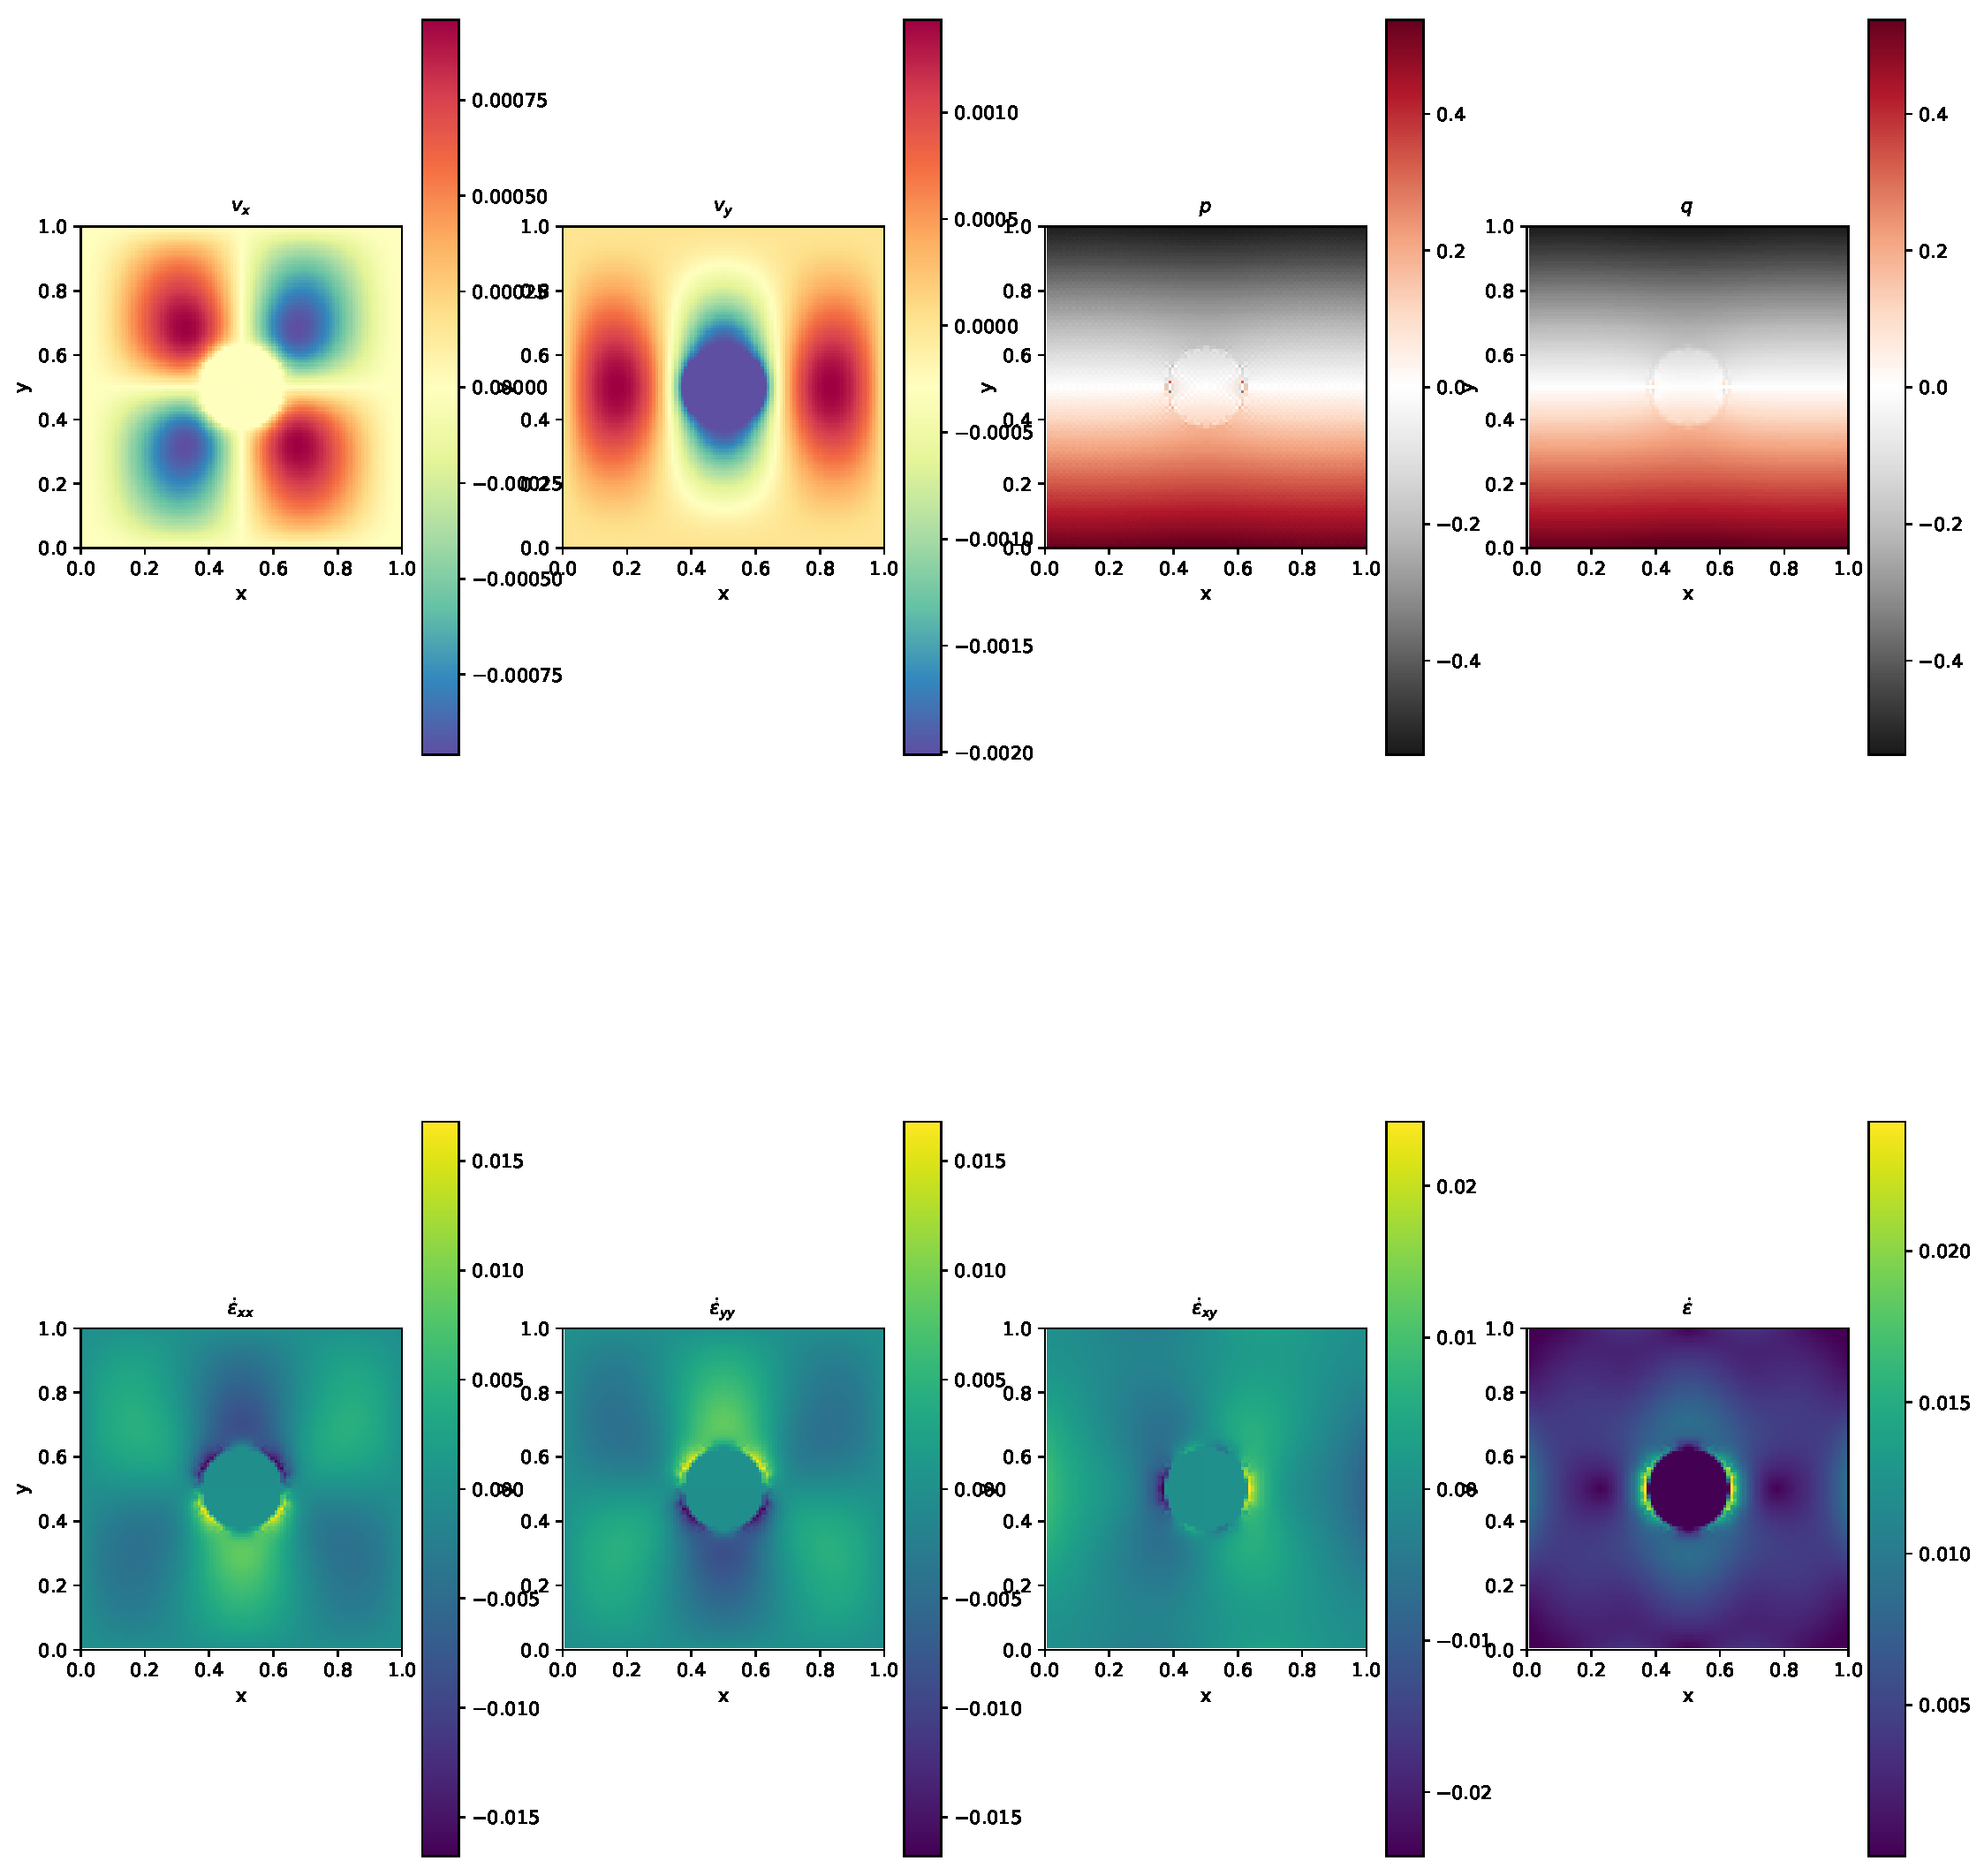
\includegraphics[width=16cm]{python_codes/fieldstone_16/solution.pdf}

The normalised residual (see {\bf solver\_pcg}) was recorded. We see that 
all things equal the resolution has a strong influence on the number of iterations the solver must
perform to reach the required tolerance. 
However, we see that the use of the preconditioner can substantially reduce the number 
of iterations inside the Stokes solver. At resolution 128x128, this number is halved. 

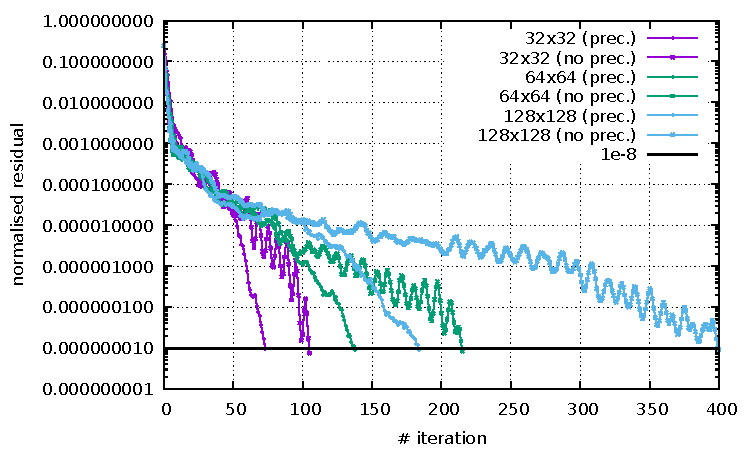
\includegraphics[width=16cm]{python_codes/fieldstone_16/images/residual.pdf}
 

